\chapter{Detecção e Prevenção de ataques port scan em redes SDN}
\label{cap:metodologia}

O objetivo principal deste trabalho é apresentar um \gls{ips} baseado em anomalia que com agrupamento de dados possa efetuar a detecção de intrusão, com foco em ataques de varredura de porta, e prover medidas de proteção contra os mesmos. Para isto, a solução foi desenvolvida considerando um ciclo de vida de três etapas (Figura \ref{fig:lifecicle}): A primeira refere-se à coleta, por parte do controlador, de informações presentes nas tabelas de fluxo dos \textit{switches} OpenFlow. A segunda etapa, de detecção, tem por finalidade a análise das informações coletadas, decidir se um fluxo é ou não malicioso e disponibilizar as informações ao controlador para que este tome as ações necessárias para prevenir o ataque. Por fim, na etapa de reação, são implementadas contramedidas para o bloqueio de ataques. Nesta etapa o controlador envia regras, definidas conforme os dados analisados, para atualização das tabelas de encaminhamento nos \textit{switches} OpenFlow. Cada uma dessas etapas será discutida no decorrer deste capítulo.

\begin{figure}[H]
  \centering
  \caption{Ciclo de vida do IPS proposto}
  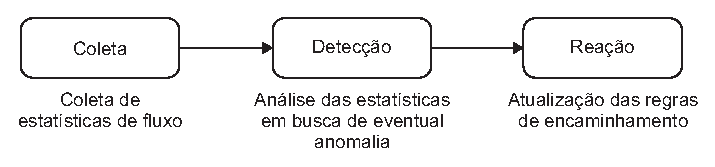
\includegraphics[width=.650\textwidth]{images/lifecicle.eps}
  \label{fig:lifecicle}
  \fonte{\footnotesize{Elaborado pelo autor.}}
\end{figure}

Este capítulo está organizado da seguinte forma: na seção \ref{sec:arq-prop} é apresentado à arquitetura do sistema desenvolvido, na seção \ref{sec:coleta} é abordada a forma de monitoramento e obtenção de estatísticas presentes na tabela de fluxo por parte do controlador. Na seção \ref{sec:deteccao} diferentes algoritmos são discutidos de forma a analisar e detectar padrões de anomalia na rede. Por fim, na seção \ref{sec:reacao}, ações de contramedida são abordadas com o objetivo de prevenir e combater atividades maliciosas na rede.

\FloatBarrier
\section{Arquitetura}
\label{sec:arq-prop}

Este trabalho  possui uma arquitetura de \gls{ips} implementada para \gls{sdn} e utiliza o protocolo OpenFlow para possibilitar a construção de um \gls{ips} distribuído. Por atuar sobre \gls{sdn}, o controlador possui visão global da rede podendo, ao detectar uma ameaça, efetuar o bloqueio de um fluxo malicioso logo na sua origem.
Esta aplicação foi desenvolvida como uma extensão do controlador OpenDaylight \cite{website:odl} fazendo parte do mesmo. 
Na arquitetura desenvolvida, o controlador gerencia e armazena as regras que definem o encaminhamento de pacotes na rede além de coletar estatísticas dos \textit{switches} OpenFlow, conforme pode ser observado na Figura \ref{fig:arch-proposta} e apresentado nas seções seguintes.

\begin{figure}
  \centering
  \caption{Fluxo de funcionamento do IPS proposto}
  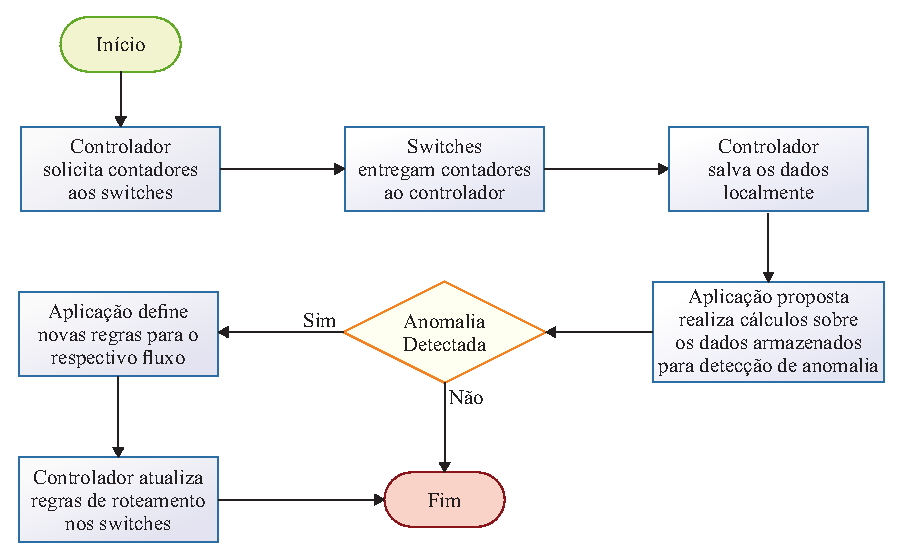
\includegraphics[width=.90\textwidth]{images/fluxo-arq.eps}
  \label{fig:arch-proposta}
  \fonte{Elaborado pelo autor.}
\end{figure}

\FloatBarrier
\section{Coleta de estatísticas}
\label{sec:coleta}

A fase de coleta é responsável por solicitar periodicamente estatísticas de fluxo dos \textit{switches} com suporte à OpenFlow e disponibilizar as informações coletadas para a etapa de detecção. Como já discutido na Seção \ref{sec:seguranca}, a análise de fluxo pode ser realizada utilizando dados dos pacotes como endereços \gls{ip} de origem e destino, ou através da análise de \textit{logs} de dispositivos. Tradicionalmente, para análise dos dados dos pacotes, várias técnicas diferentes de monitoramento são utilizadas. Cada técnica de monitoramento requer uma instalação separada de hardware ou configuração de software, tornando isso moroso e com custo alto de implementação. No entanto, OpenFlow  provê as interfaces necessárias para implementar a maioria dos métodos discutidos, sem a necessidade de grandes customizações \cite{Adrichem:2014}.

A definição do intervalo de coleta das entradas de fluxo é de grande importância. Se a coleta é realizada com períodos muito grandes, haverá um atraso na detecção de ataques. Por outro lado, se o intervalo for curto demais, haverá um aumento de tráfego referente às requisições de coleta. Neste trabalho este intervalo foi definido em três segundos com base em resultados obtidos em testes realizados. Este período não produz grande carga na rede e possibilita que várias tentativas de varredura de porta possam ser realizadas, obtendo-se mais fluxos distintos a cada coleta. Também foi adicionado um \textit{timeout} de quinze segundos para os fluxos registrados na tabela de encaminhamento, com isso, a frequência na consulta também permite que as estatísticas de fluxo sejam atualizadas com maior frequência. Apesar desse intervalo possibilitar uma grande quantidade de varreduras antes que as mesmas sejam detectadas, o fato de prover um bloqueio posterior impossibilita que o atacante efetue outros ataques ao término da varredura.

Utilizando as mensagens definidas pelo protocolo OpenFlow e brevemente discutidas na seção \ref{subsec:protocolo-comunicacao}, a coleta de estatísticas é facilitada, passando a ser feita pelo controlador da rede. O controlador realiza, através do protocolo OpenFlow, a coleta de contadores presentes nas tabelas de fluxo dos \textit{switches}. Esses contadores foram definidos com o objetivo de facilitar a criação de mecanismos de \gls{qos} \cite{website:onf} e possuem informações agrupadas por fluxo, por porta, etc. e serão a fonte de informação para este trabalho.

Analisando o que foi discutido na seção \ref{sec:varredura}, técnicas para detecção de varredura de portas podem facilmente ser implementadas utilizando informações do cabeçalho dos pacotes e que também estão presentes nas tabelas de fluxo, como \textit{host} de origem e destino e portas de destino. A fim de se obter estatísticas referentes aos fluxos, OpenFlow fornece alguns métodos para obtenção de informações detalhadas de um fluxo específico, ou de um conjunto de fluxos.

Segundo a especificação OpenFlow \cite{OpenFlowSpec:2014} se o controlador desejar obter estatísticas de um fluxo OpenFlow, ele deve enviar uma mensagem \textit{multipart} (ofp\_multipart\_request) do tipo OFPMP\_FLOW para o \textit{switch}. Mensagens \textit{multipart} são usadas para codificar pedidos ou respostas que podem carregar grande quantidade de informações que nem sempre se encaixam em uma única mensagem OpenFlow, que é limitada a 64KB. O pedido ou resposta é codificada como uma sequência de mensagens de várias partes de determinado tipo em uma mesma conexão, e remontadas pelo receptor. Cada sequência de mensagens \textit{multipart}, carrega apenas uma solicitação ou resposta. Mensagens \textit{multipart} são comumente utilizadas para solicitações de estatísticas ou informações do \textit{switch} \cite{OpenFlowSpec:2014}.

O corpo (\textit{payload}) da mensagem de requisição deve ser preenchido segundo o formato exibido pela Figura \ref{fig:ofp-multipart-request} a seguir:

\begin{figure}[H]
  \centering
  \caption{Estrutura do corpo da mensagem de solicitação de estatísticas}
  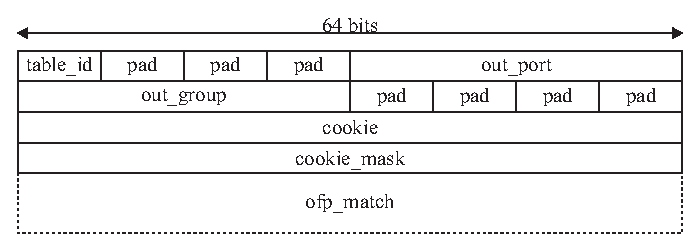
\includegraphics[width=.80\textwidth]{images/ofp-flow-stats-request.eps}
  \label{fig:ofp-multipart-request}
  \fonte{Elaborado pelo autor a partir de\\informações da especificação OpenFlow.}
\end{figure}

O campo \textit{table\_id} deve ser preenchido com o número da tabela onde os fluxos desejados estão armazenados. Se o controlador desejar obter estatísticas de todos os fluxos dessa tabela, apenas essa informação é obrigatória, caso contrário, se o controlador desejar estatísticas de um fluxo específico, devem ser preenchidos os campos de \textit{match}, como endereço de origem e porta destino. Os campos \textit{pad} não necessitam de informação, servem apenas para completar o pacote.

Após enviar a mensagem de requisição, o controlador deve esperar por uma resposta da mensagem pelo \textit{switch}. Se a resposta exceder o limite máximo da mensagem OpenFlow (64KB) o \textit{switch} então, irá enviar uma sequência de múltiplas mensagens com a \textit{flag} OFPMP\_REPLY\_ MORE no cabeçalho da mensagem \textit{multipart} habilitada. 

Se o controlador recebe a mensagem de resposta com esta \textit{flag} habilitada, ele deve armazenar a sequência de mensagens até que a última mensagem da sequência seja recebida. Como o \textit{switch} envia a sequência de mensagens de várias partes com o mesmo ID de transação (xid), o controlador deve mapear todas as partes na sequência e deve ler a mensagem para obter as informações estatísticas.

Quando o \textit{switch} recebe a mensagem OFPMP\_FLOW, ele primeiramente obtém a entrada do fluxo correspondente com base nos campos informados na requisição. Uma vez obtidas as entradas de fluxo correspondentes, o mesmo constrói uma mensagem de resposta (Figura \ref{fig:ofp-flow-stats}) e a envia de volta para o controlador. Esta mensagem pode ser enviada através de um ou mais pacotes, dependendo do tamanho da mesma.

\begin{figure}[H]
  \centering
  \caption{Corpo da resposta à requisição OFPMP\_FLOW.}
  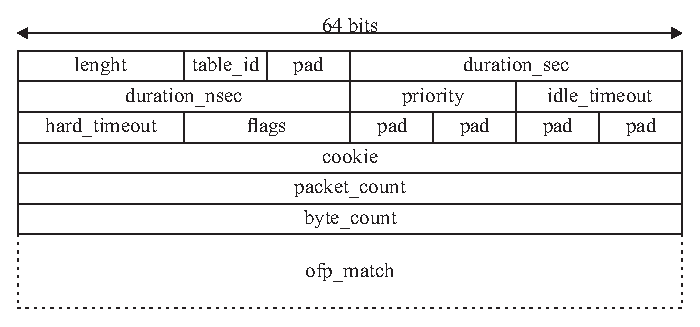
\includegraphics[width=.80\textwidth]{images/ofpmp-flow-stats.eps}
  \label{fig:ofp-flow-stats}
  \fonte{Elaborado pelo autor a partir de informações da especificação OpenFlow.}
\end{figure}

\begin{itemize}
    \item \textit{lenght} indica o tamanho da respectiva entrada de fluxo;
    \item \textit{table\_id} refere-se ao identificador da tabela cujo fluxo foi solicitado;
    \item \textit{duration\_sec} e \textit{duration\_nsec} indicam o tempo decorrido do fluxo desde sua entrada no \textit{pipeline} OpenFlow. A duração total em nano segundos pode ser obtido pelo cálculo $duration\_sec * 10^9 + duration\_nsec$;
    \item \textit{flags} possui informações das \textit{flags} TCP como SYN, ACK e FIN;
    \item \textit{packet\_count} é um contador de medição de pacotes que trafegam com o respectivo \textit{match} desse fluxo;
    \item \textit{byte\_count} indica o número de \textit{bytes} do respectivo fluxo; e
    \item \textit{ofp\_match} é uma lista de zero ou mais propriedades específicas para as regras, como portas de origem e destino, tipo de rede, endereços de origem e destino, etc.
\end{itemize}


O controlador OpenDaylight implementa uma abstração dos pacotes e protocolos utilizados, tornando a tarefa de desenvolver troca de mensagens com os \textit{switches} mais ágil e prática.
A sua estrutura de funcionamento é baseada em uma árvore, o que possibilita o endereçamento de qualquer elemento/sub-árvore que esteja sob o domínio do controlador. Nesta árvore, ilustrada na Figura \ref{fig:arvore-dados}, tem-se o controlador interligado aos \textit{switches}, que por sua vez possuem tabelas e estes, possuem nodos que correspondem às informações de fluxos. Sendo assim, pode-se obter estatísticas de fluxo de um determinado \textit{switch} através da leitura sucessiva de seus nodos. Para obter as estatísticas do primeiro fluxo presente da segunda tabela do primeiro \textit{switch}, deve realizar a leitura do nodo "\textit{Switch} 1", a partir deste nodo pode-se realizar uma leitura de todas as tabelas presentes até que se encontre a "Tabela 2", estando na tabela dois pode-se obter as estatísticas agregadas de fluxo ou de fluxos específicos, que neste exemplo é o "Fluxo 1".

\begin{figure}[H]
  \centering
  \caption{Representação da árvore de dados no OpenDaylight.}
  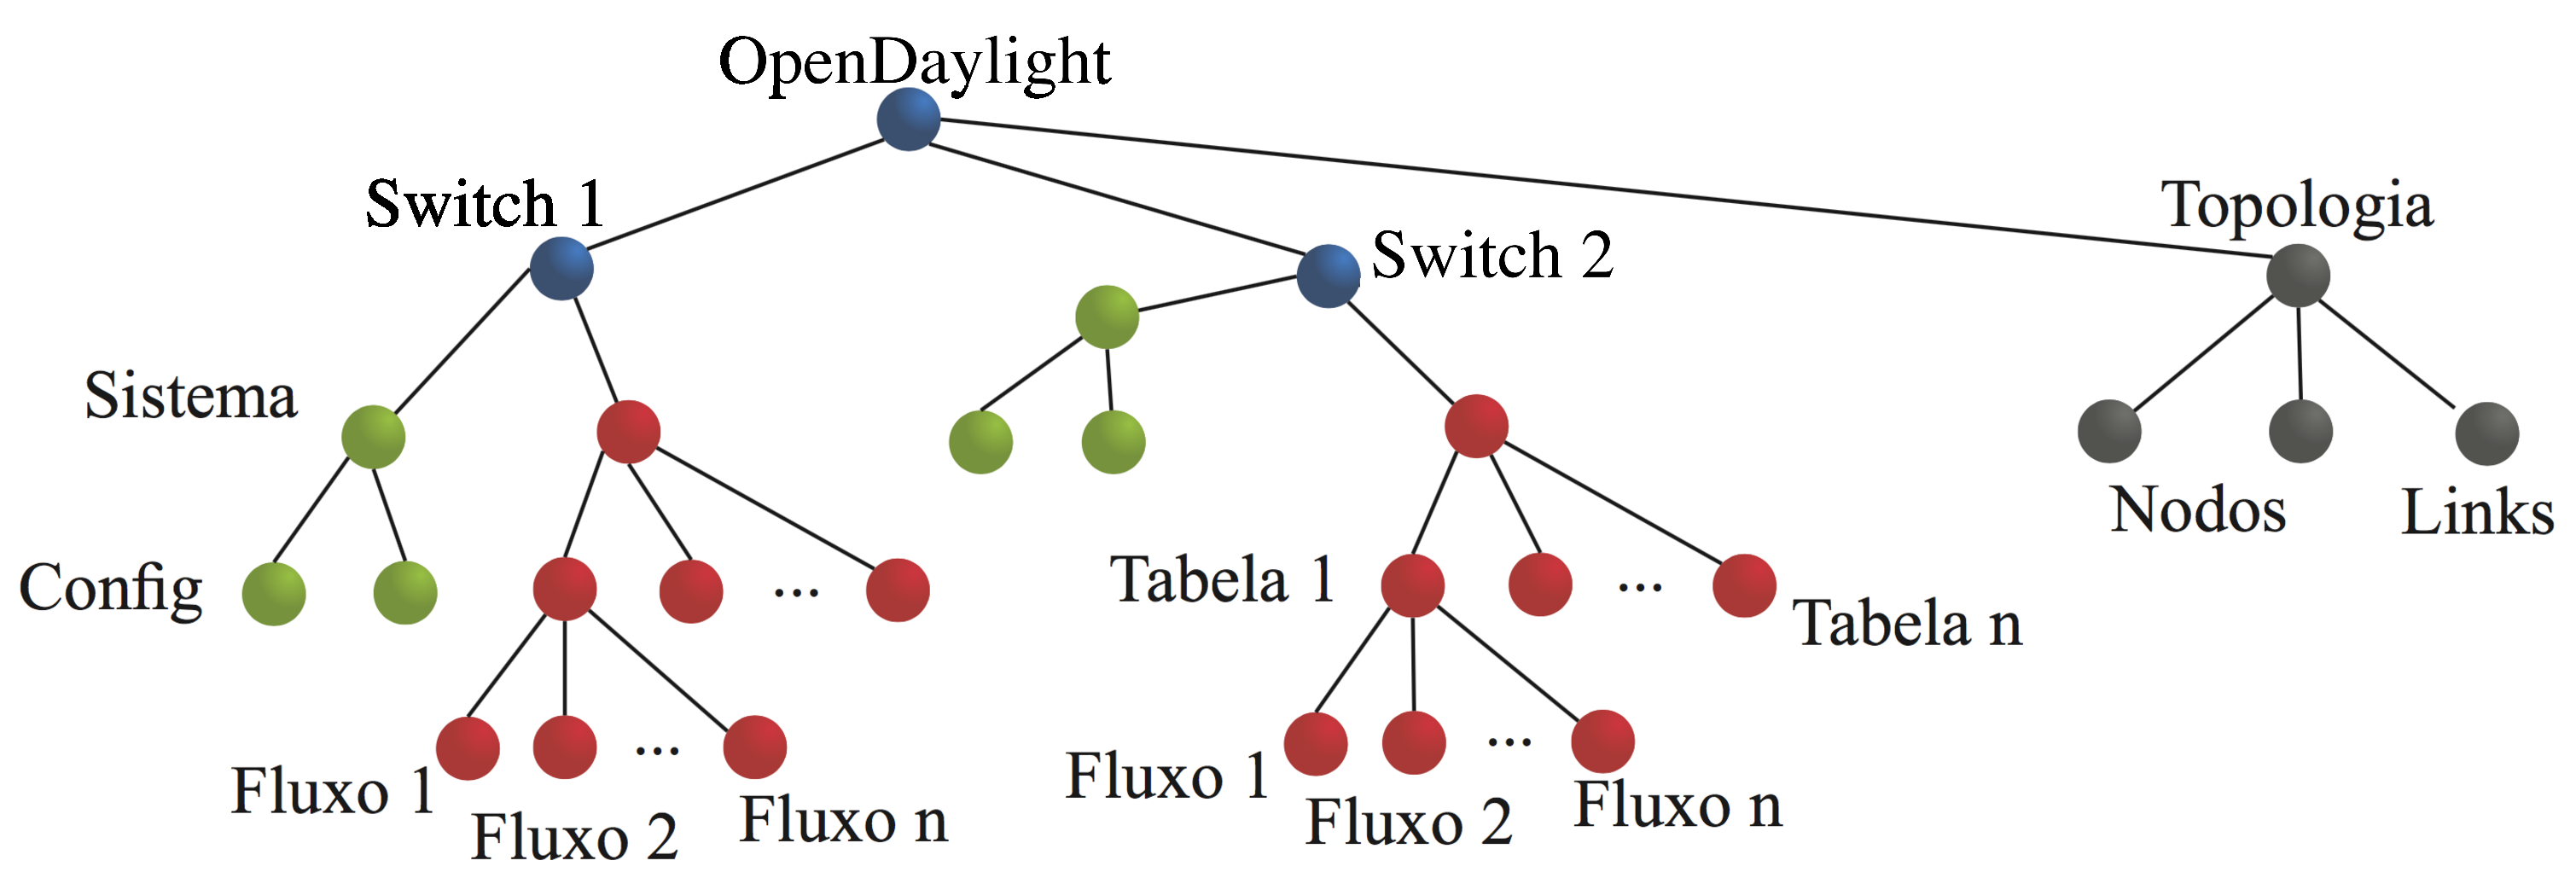
\includegraphics[width=.9\textwidth]{images/arvore.eps}
  \label{fig:arvore-dados}
  \fonte{\centering Elaborado pelo autor com base na especificação OpenDaylight.}
\end{figure}

A configuração dos dispositivos e a coleta de estatísticas de fluxos no OpenDaylight pode ser obtida de forma muito simples através de um \textit{browser} utilizando-se uma \gls{api} chamada \textit{restconf}. Um exemplo de requisição de estatística de fluxo pode ser obtida através do Localizador Uniforme de Recursos (\gls{url}): http://localhost/restconf/config/open- daylight-inventory:nodes/node/openflow:1/table/0/flow/tcipsflow-1

Onde:
\begin{itemize}
    \item http://localhost - é o endereço \gls{web} do controlador;
    \item restconf - é o nome da \gls{api} ao qual está se requisitando a informação;
    \item config - é a base de dados de configuração do OpenDaylight;
    \item opendaylight-inventory:nodes - indica que a partir desse ponto a estrutura é baseada em nodos;
    \item nodo/openflow:1 - indica que o nodo a ser consultado é o chamado openflow:1;
    \item table/0 - indica que a tabela do nodo acima a ser consultada é a de identificação 0; e
    \item flow/tcipsflow-1 - indica que o fluxo de nome "tcipsflow-1" deverá ser consultada na tabela acima.
\end{itemize}

Se o desejado for obter a informação de todos os fluxos da tabela, a informação de fluxo  (\textit{flow}) pode ser omitida da \gls{url}, como por exemplo: http://localhost/restconf/config/openday- light-inventory:nodes/node/openflow:1/table/0. O resultado será um arquivo em formato \gls{json} ou \gls{xml} como exibido na Figura \ref{cod:ofp-flow-stats}.
\begin{figure}[H]
  \centering
  \caption{Corpo da resposta ofp-flow-stats no formato JSON}
\begin{lstlisting}[belowskip=-0.05 \baselineskip]
{ "flow-node-inventory:table": [
    {"id": 0,
      "opendaylight-flow-table-statistics:flow-table-statistics": {
        "packets-looked-up": 37,
        "active-flows": 3,
        "packets-matched": 19 },
      "flow": [
        { "id": "tcipsflow-1",
          "table_id": 0,
          "instructions": {
            "instruction": [
              { "order": 0,
                "apply-actions": {
                  "action": [
                    { "order": 0,
                      "output-action": {
                        "output-node-connector": "CONTROLLER"}}]}}]},
          "priority": 1,
          "opendaylight-flow-statistics:flow-statistics": {
            "duration": { "nanosecond": 583000000, "second": 156 },
            "packet-count": 1, 
            "byte-count": 74 },
          "match": {
            "ethernet-match": { "ethernet-type": { "type": 2048 }},
            "ip-match": { "ip-protocol": 6 }},
          "idle-timeout": 0,
          "hard-timeout": 0 }]}]}
\end{lstlisting}
\fonte{\centering Extraido da interface do OpenDaylight executado pelo autor.}
 \label{cod:ofp-flow-stats}
 \end{figure}
Neste exemplo, cada nodo é representado por um sub-elemento JSON. A tabela possui dados agregados de pacotes transmitidos e fluxos. Cada fluxo por sua vez possui informações de \textit{match} para a verificação do pacote recebido, \textit{instructions}, instruções que devem ser tomadas se os campos em \textit{match} forem satisfeitos, campos de \textit{timeout}, \textit{flags} e estatísticas conforme o especificado pelo protocolo Openflow.
 
Apesar de a coleta ser facilmente realizada através da \gls{api} \textit{restconf}, esta aplicação implementa a coleta diretamente sobre a base de dados do controlador, fazendo uso dos métodos desenvolvidos pela comunidade de desenvolvedores do OpenDaylight. Esta escolha torna-se mais viável considerando-se que esta aplicação foi desenvolvida como uma parte do controlador, tendo portanto, acesso direto à sua base de dados e dispositivos. Na Figura \ref{cod:code-colection} é ilustrada a obtenção de um fluxo diretamente da base de dados OpenDaylight. Neste exemplo cada elemento da árvore deve ser verificado até que o nodo que contém informações de fluxo seja encontrado.

\begin{figure}[H]
  \centering
  \caption{Exemplo para obtenção de estatísticas da base de dados do OpenDaylight}
\begin{lstlisting}[belowskip=-0.05 \baselineskip]
Nodos nodos = obterNodosDaBaseDeDados();
/* Iteracao sobre cada nodo */
for (Iterator<Node> iterator = nodes.getNode().iterator(); 
    iterator.hasNext();) {
  
  Node childNode = iterator.next();
  /* Iteracao sobre cada tabela */
  for (Iterator<Table> iterator2 = childNode.getTable().iterator();
  iterator2.hasNext();) {
    
    Table table = iterator2.next();
    /* Iteracao sobre cada fluxo */
    for (Iterator<Flow> iterator3 = table.getFlow().iterator(); 
    iterator3.hasNext();) {
      
      Flow flow = iterator3.next();
      /* Obtem dados do cabecalho - match */
      Match match = flow.getMatch();
      Layer3Match layer3Match = match.getLayer3Match();
      Layer4Match layer4Match = match.getLayer4Match();
      ...
      /* Obtem estatisticas */
      FlowStatisticsData data = flow.getAugmentation(
        FlowStatisticsData.class);
      FlowStatistics flowStatistics = data.getFlowStatistics();
      /* Salva informacoes para posterior analise */
      setMatch(match);
      setPacketCount(flowStatistics.getPacketCount().getValue());
      setByteCount(flowStatistics.getByteCount().getValue());
      setDurationSeconds(flowStatistics.getDuration().getSecond()
        .getValue());
      setDurationNanoSeconds(flowStatistics.getDuration().getNanosecond()
        .getValue());
    }
  }
}
\end{lstlisting}
\label{cod:code-colection}
\fonte{\centering Elaborado pelo autor.}
\end{figure}

A base de dados criada para armazenar as estatísticas é composta por campos de \textit{match} necessários para diferenciar os fluxos e por campos dos contadores por fluxo da tabela de encaminhamento conforme listado abaixo.

\begin{itemize}
    \item nodeName - nome do \textit{switch} analisado;
    \item etherType - o tipo de pacote recebido, neste projeto são analisados apenas pacotes TCP;
    \item srcIpv4 - o IP de origem do fluxo;
    \item dstIpv4 - o IP de destino do fluxo;
    \item srcPort - a porta de origem do fluxo;
    \item dstPort - a porta de destino do fluxo;
    \item incomeTime - o instante em que o primeiro pacote foi recebido;
    \item durationSeconds - a duração do fluxo em segundos;
    \item durationNanoSeconds - a duração do fluxo em nano segundos;
    \item packetCount - o número de pacotes do fluxo trafegados pelo \text{switch};
    \item byteCount - o número de bytes do fluxo trafegados pelo \text{switch};
\end{itemize}

Uma vez armazenadas as estatísticas de fluxo na base de dados criada, o processo de coleta é finalizado até iniciar um novo ciclo.
\section{Detecção}
\label{sec:deteccao}


Periodicamente são analisadas as informações de fluxos presentes na base de dados alimentada na coleta dos contadores. A cada análise são executadas as seguintes etapas:

\begin{itemize}
    \item Seleção dos fluxos armazenados na base de dados que possuam número de pacotes reduzido, característico de fluxos de varredura de porta, e que tenham sido gerados nos últimos segundos;
    \item Agrupamento dos fluxos selecionados, por endereço de origem e destino e porta de destino;
    \item Obtenção da quantidade de fluxos com endereços de origem e destino semelhantes em um pequeno intervalo de tempo predefinido. Eventuais tentativas de varredura de porta podem ocorrer em qualquer sistema, sendo assim, um único fluxo não pode gerar um evento para bloqueio.
    \item Classificação do tipo de varredura (horizontal, vertical e mista) com base nas informações de endereço de origem e destino e porta de destino.
    \item Inserção do endereço de origem em uma lista de endereços para descarte.
\end{itemize}

Em geral, fluxos de tentativas de varredura de porta limitam-se em no máximo três pacotes, por exemplo \textit{TCP Connect} possui pacotes SYN, SYN/ACK e ACK, com exceção dos caso onde há retransmissão de pacotes devido à perdas. Além disso, estatisticamente, ataques do tipo \textit{port scan} ocorrem em intervalos pequenos de tempo, em média menos de um minuto. É sobre esse conjunto de fatores que a aplicação foi desenvolvida.

Como há uma coleta periódica das estatísticas de fluxo, é possível analisar se houve aumento no número de pacotes entre uma consulta e outra. Para definir se um fluxo é considerado varredura, neste projeto foi estabelecido um número máximo de cinco pacotes para o mesmo. Este número corresponde aos três pacotes responsáveis pelo \textit{handshake} da conexão com uma tolerância de dois pacotes em caso de retransmissão. Por este número de pacotes ser baixo, a probabilidade de se ter um fluxo não malicioso detectado como varredura é muito baixa.

\subsection{Detecção de varredura horizontal}

A detecção de varredura horizontal de portas é desenvolvido pela premissa de que vários fluxos, para uma mesma porta em diferentes \textit{hosts} alvo são originadas de um mesmo \textit{host} de origem. Nesse tipo de intrusão a aplicação desenvolvida analisa a origem e o destino das conexões. 

Endereços \gls{ip} de origem, que possuam fluxos pequenos e que estejam tentando conectar-se à no mínimo três \textit{hosts} em uma mesma porta, são consideradas anomalias. Assim, o endereço de origem é adicionado na lista de endereços para descarte.

\subsection{Detecção de varredura vertical}

Na detecção de varredura vertical, tem-se a premissa de que um \textit{host} de origem realiza a varredura de várias portas em um mesmo \textit{host} de destino. Neste caso, \textit{hosts} de origem que possuam inúmeros fluxos para diferentes portas, podem ser reconhecidos pela aplicação como uma anomalia. Para esta classificação foi criada uma verificação com base em pesos. Portas que em geral sofrem mais com a varredura, como as de servidores de aplicação e de arquivos, possuem um peso maior sobre as demais portas. Quando a soma dos pesos de cada fluxo ultrapassar um limiar predefinido, é caracterizado um ataque de varredura. 

Neste projeto foi estabelecido um peso cinco para portas com maior probabilidade de varredura (portas previamente definidas em 22, 23, 25, 80, 5432, 8080) e peso três para as demais portas. Quando a soma de pesos dos fluxos de mesma origem e destino ultrapassar o limiar estabelecido em quinze, um ataque de varredura pode ter sido realizado, sendo assim, é inserido seu endereço na lista de endereços para descarte.

\subsection{Detecção de varredura \textit{block}}

Nesse tipo de varredura, ambas as premissas já citadas devem ser consideradas. Neste, a aplicação proposta realiza a verificação de \textit{hosts} de origem que tentam estabelecer conexões em no mínimo dois \textit{hosts}. 

No mínimo um destes \textit{hosts} também devem apresentar uma soma de pesos de varredura vertical estabelecido em seis. Resumindo, se dois \textit{hosts} tiverem determinada porta verificada e ao menos um deles tiver uma porta distinta verificada, é considerado um ataque de varredura.



\section{Ações de reação}
\label{sec:reacao}

Inicialmente, todos os comutadores possuem suas tabelas de encaminhamento vazias. Sendo assim, ao receber um pacote ocorre um \textit{table miss} e o pacote é encaminhado para o controlador através de uma mensagem \textit{Packet In}.

O controlador por si só, não realiza operações sobre a mensagem recebida, por isso, foi desenvolvido juntamente com este IPS, um interpretador de mensagens \textit{Packet In}. Este analisa os dados do cabeçalho do pacote obtendo as informações de origem e destino do fluxo e os compara com os endereços armazenados na lista de endereços maliciosos para descarte. Dependendo do resultado, o controlador poderá adicionar no \textit{switch} uma regra de encaminhamento o ou tomar uma ação de prevenção, adicionando uma regra para descarte do fluxo.

Mensagens para alteração da tabela de encaminhamento podem ter os seguintes tipos:
\begin{itemize}
    \item \textbf{OFPFC\_ADD} - Adiciona um novo fluxo;
    \item \textbf{OFPFC\_MODIFY} - Modifica entradas de fluxo existentes;
    \item \textbf{OFPFC\_MODIFY\_STRICT} - Modifica entradas de fluxo existentes validando estritamente seus campos, ou seja, apenas uma entrada da tabela é modificada;
    \item \textbf{OFPFC\_DELETE} - Remove entradas de fluxo existente; e
    \item \textbf{OFPFC\_DELETE\_STRICT} - Remove entradas de fluxo validando estritamente seus campos, ou seja, apenas uma entrada da tabela é removida.
\end{itemize}

Entradas de fluxos podem ser removidos da tabela de encaminhamento por duas maneiras: através da requisição do controlador e pelo mecanismo de \textit{timeout}. O mecanismo de \textit{timeout} é executado pelo \textit{switch} independentemente do controlador e é baseado na configuração e no estado das entradas de fluxo. Neste trabalho, foi definido um intervalo de \textit{timeout} para cada fluxo para que não ocorra \textit{overflow} de regras nas tabelas de encaminhamento. Um fluxo só permanecerá na tabela por intervalo de quinze segundos após o recebimento de seu último pacote, com exceção para as entradas de fluxo para descarte, nestes o \textit{timeout} foi definido em zero a fim de prover a proteção até que o administrador, manualmente, o remova da tabela.

Para alterar ou remover alguma entrada da tabela de fluxo, deve ser enviada uma mensagem do tipo OFPT\_FLOW\_MOD que é definida conforme ilustra a Figura \ref{fig:ofp-flow-mod}.

\begin{figure}[H]
  \centering
  \caption{Corpo da mensagem de alteração de entradas na tabela de fluxo.}
  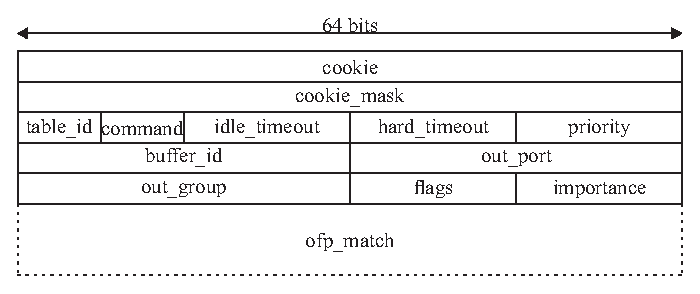
\includegraphics[width=.80\textwidth]{images/ofp-flow-mod.eps}
  \label{fig:ofp-flow-mod}
  \fonte{\centering Elaborado pelo autor a partir de informações da especificação OpenFlow.}
\end{figure}
O campo \textit{table\_id} refere-se à tabela a ser atualizada, que pode ser por fluxo, porta, como já citado. O campo \textit{command} refere-se á ação a ser executada (adição, alteração e remoção), campos \textit{timeout} indicam o tempo máximo de espera por um fluxo antes do descarte, \textit{priority} armazena a prioridade da entrada na tabela de fluxo. O campo \textit{ofp\_match} indicam as regras de encaminhamento de fluxos. Os demais campos não serão abordados neste mas seu estudo pode ser realizado através especificação OpenFlow \cite{OpenFlowSpec:2014}.

Alterando a regras de encaminhamento através destas mensagens, além de reagir ao ataque em questão, o sistema também estará protegido contra novos fluxos de mesma origem, sem a necessidade de consultar o controlador.

Algumas medidas de prevenção também foram preestabelecidas no controlador. Por padrão toda conexão não maliciosa, deve iniciar a comunicação com um pacote SYN. Sendo assim, ao receber um pacote com \textit{flag} diferente da SYN, o controlador imediatamente descarta o pacote, prevenindo assim o ataques do tipo ACK, exploração FIN e Xmas Tree.

Os fluxos adicionados pelo controlador nas tabelas de encaminhamento possuem como regras as informações chave do cabeçalho mencionadas, desta forma, cada fluxo recebido irá possuir uma única entrada na tabela. Neste instante é também configurado um \textit{timeout} para este fluxo. Este \textit{timeout} foi estabelecido em quinze segundos, tempo permite que o fluxo não seja removido da tabela caso houver um pequeno atraso na transmissão dos pacotes além de possibilitar que coletas de estatísticas sejam realizadas, pois uma vez removido o fluxo, não é mais possível obter suas informações. O Quadro \ref{fll}, ilustra uma tabela de fluxo com as regras utilizadas pelo \textit{software} proposto, regras não utilizadas foram omitidas da tabela para melhor leitura.

\begin{table}[H]
\centering
\caption{Exemplo de fluxos na tabela de encaminhamento.}
\resizebox{\textwidth}{!}{
\label{fll}
\begin{tabular}{|c|c|c|c|c|c|c|c|}
\hline
\multicolumn{5}{|c|}{REGRAS}                           & AÇÃO       & PRIORIDADE & TIMEOUT       \\ \hline
type & src\_ip    & dst\_ip    & src\_port & dst\_port &            &            & idle\_timeout \\ \hline
TCP  & 10.0.0.11  & 10.0.1.124 & 36987     & 80        & encaminhar & 50000      & 15            \\ \hline
TCP  & 10.10.0.45 & 10.10.2.43 & 23234     & 80        & encaminhar & 50000      & 15            \\ \hline
TCP  & 10.0.0.114 & 10.10.2.29 & 35455     & 22        & encaminhar & 50000      & 15            \\ \hline
TCP  & 10.10.2.24 & 10.0.0.12  & 32444     & 25        & descartar  & 50000      & 0             \\ \hline
\end{tabular}}
\fonte{\centering Elaborado pelo autor.}
\end{table}

Neste exemplo, os três primeiros fluxos são de encaminhamento e foram criados com um \textit{idle\_timeout} de quinze segundo. Se nenhum novo pacote desse fluxo for recebido nesse intervalo de tempo, o fluxo é removido da tabela de encaminhamento. O quarto fluxo é de descarte, ou seja, quando for recebido um fluxo onde os campos de cabeçalho dos pacotes correspondam aos campos das regras, o mesmo será descartado. Este último possui um \textit{timeout} nulo, o que significa que a regra é permanente e, se necessário for, deverá ser removida da tabela através de uma mensagem do controlador.

A natureza de visão global da rede possibilitada por \gls{sdn} permite que a aplicação faça a detecção de \text{switches} individuais e envie fluxos de descarte para os demais, impossibilitando que tais fluxos tomem rotas diferentes para o \textit{host} alvo. Além disso, controladores distintos podem efetuar a troca de informações referentes a fluxos de varredura de porta, possibilitando a proteção de outras redes não gerenciadas pelo mesmo controlador.










%Should I write about Statistical Problems with Statistical-based Intrusion Detection?